\newpage
\subsection{Teacher Page}
The Teacher page is divided into four sections: “dashboard”, “List of Students”, “Post Materials” and “Receive Queries”. The main area of the dashboard section contains the total number of students enrolled for each course details.\\

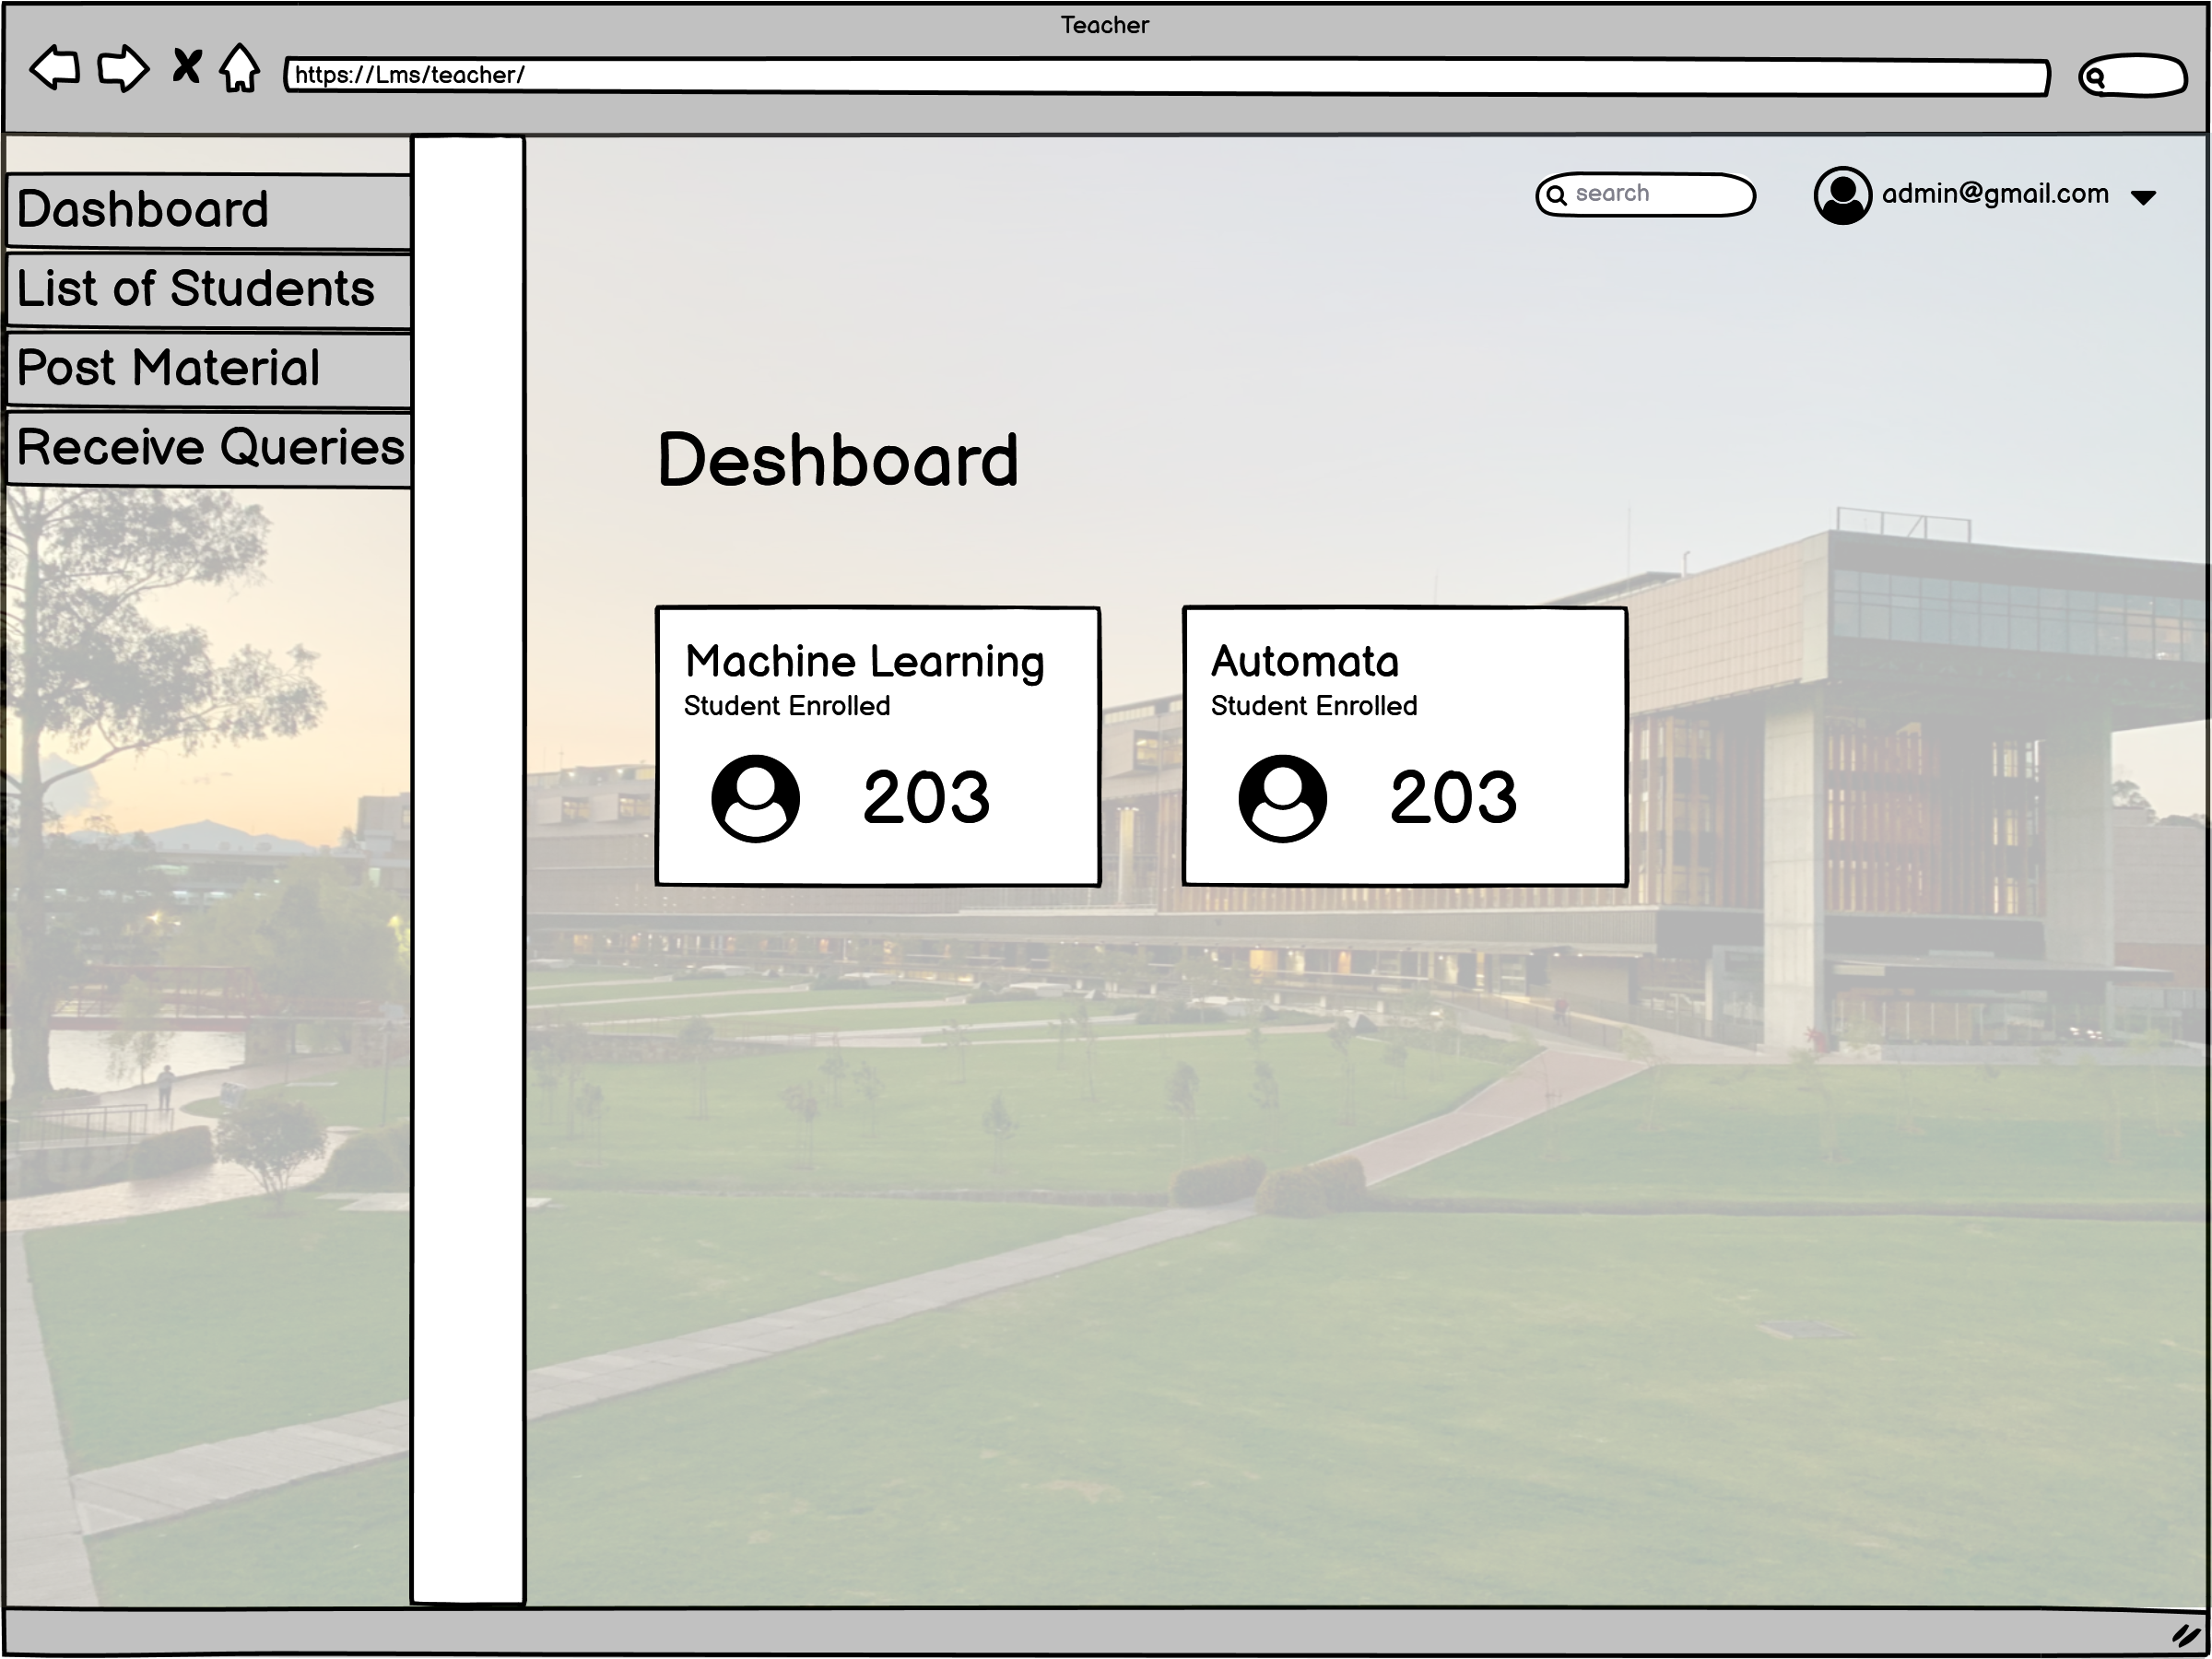
\includegraphics[width=\columnwidth]{images/Teacher Deshboard.png}
\newpage
The “List of Students” section contains a table  with all the information about each student and also there is a “Modify” column where teacher can update or delete data.  Clicking on the button “update” teacher updates the user details, or the button “delete” teacher deletes the user from the database, revoking their possibility to login and therefore to access the courses.\\

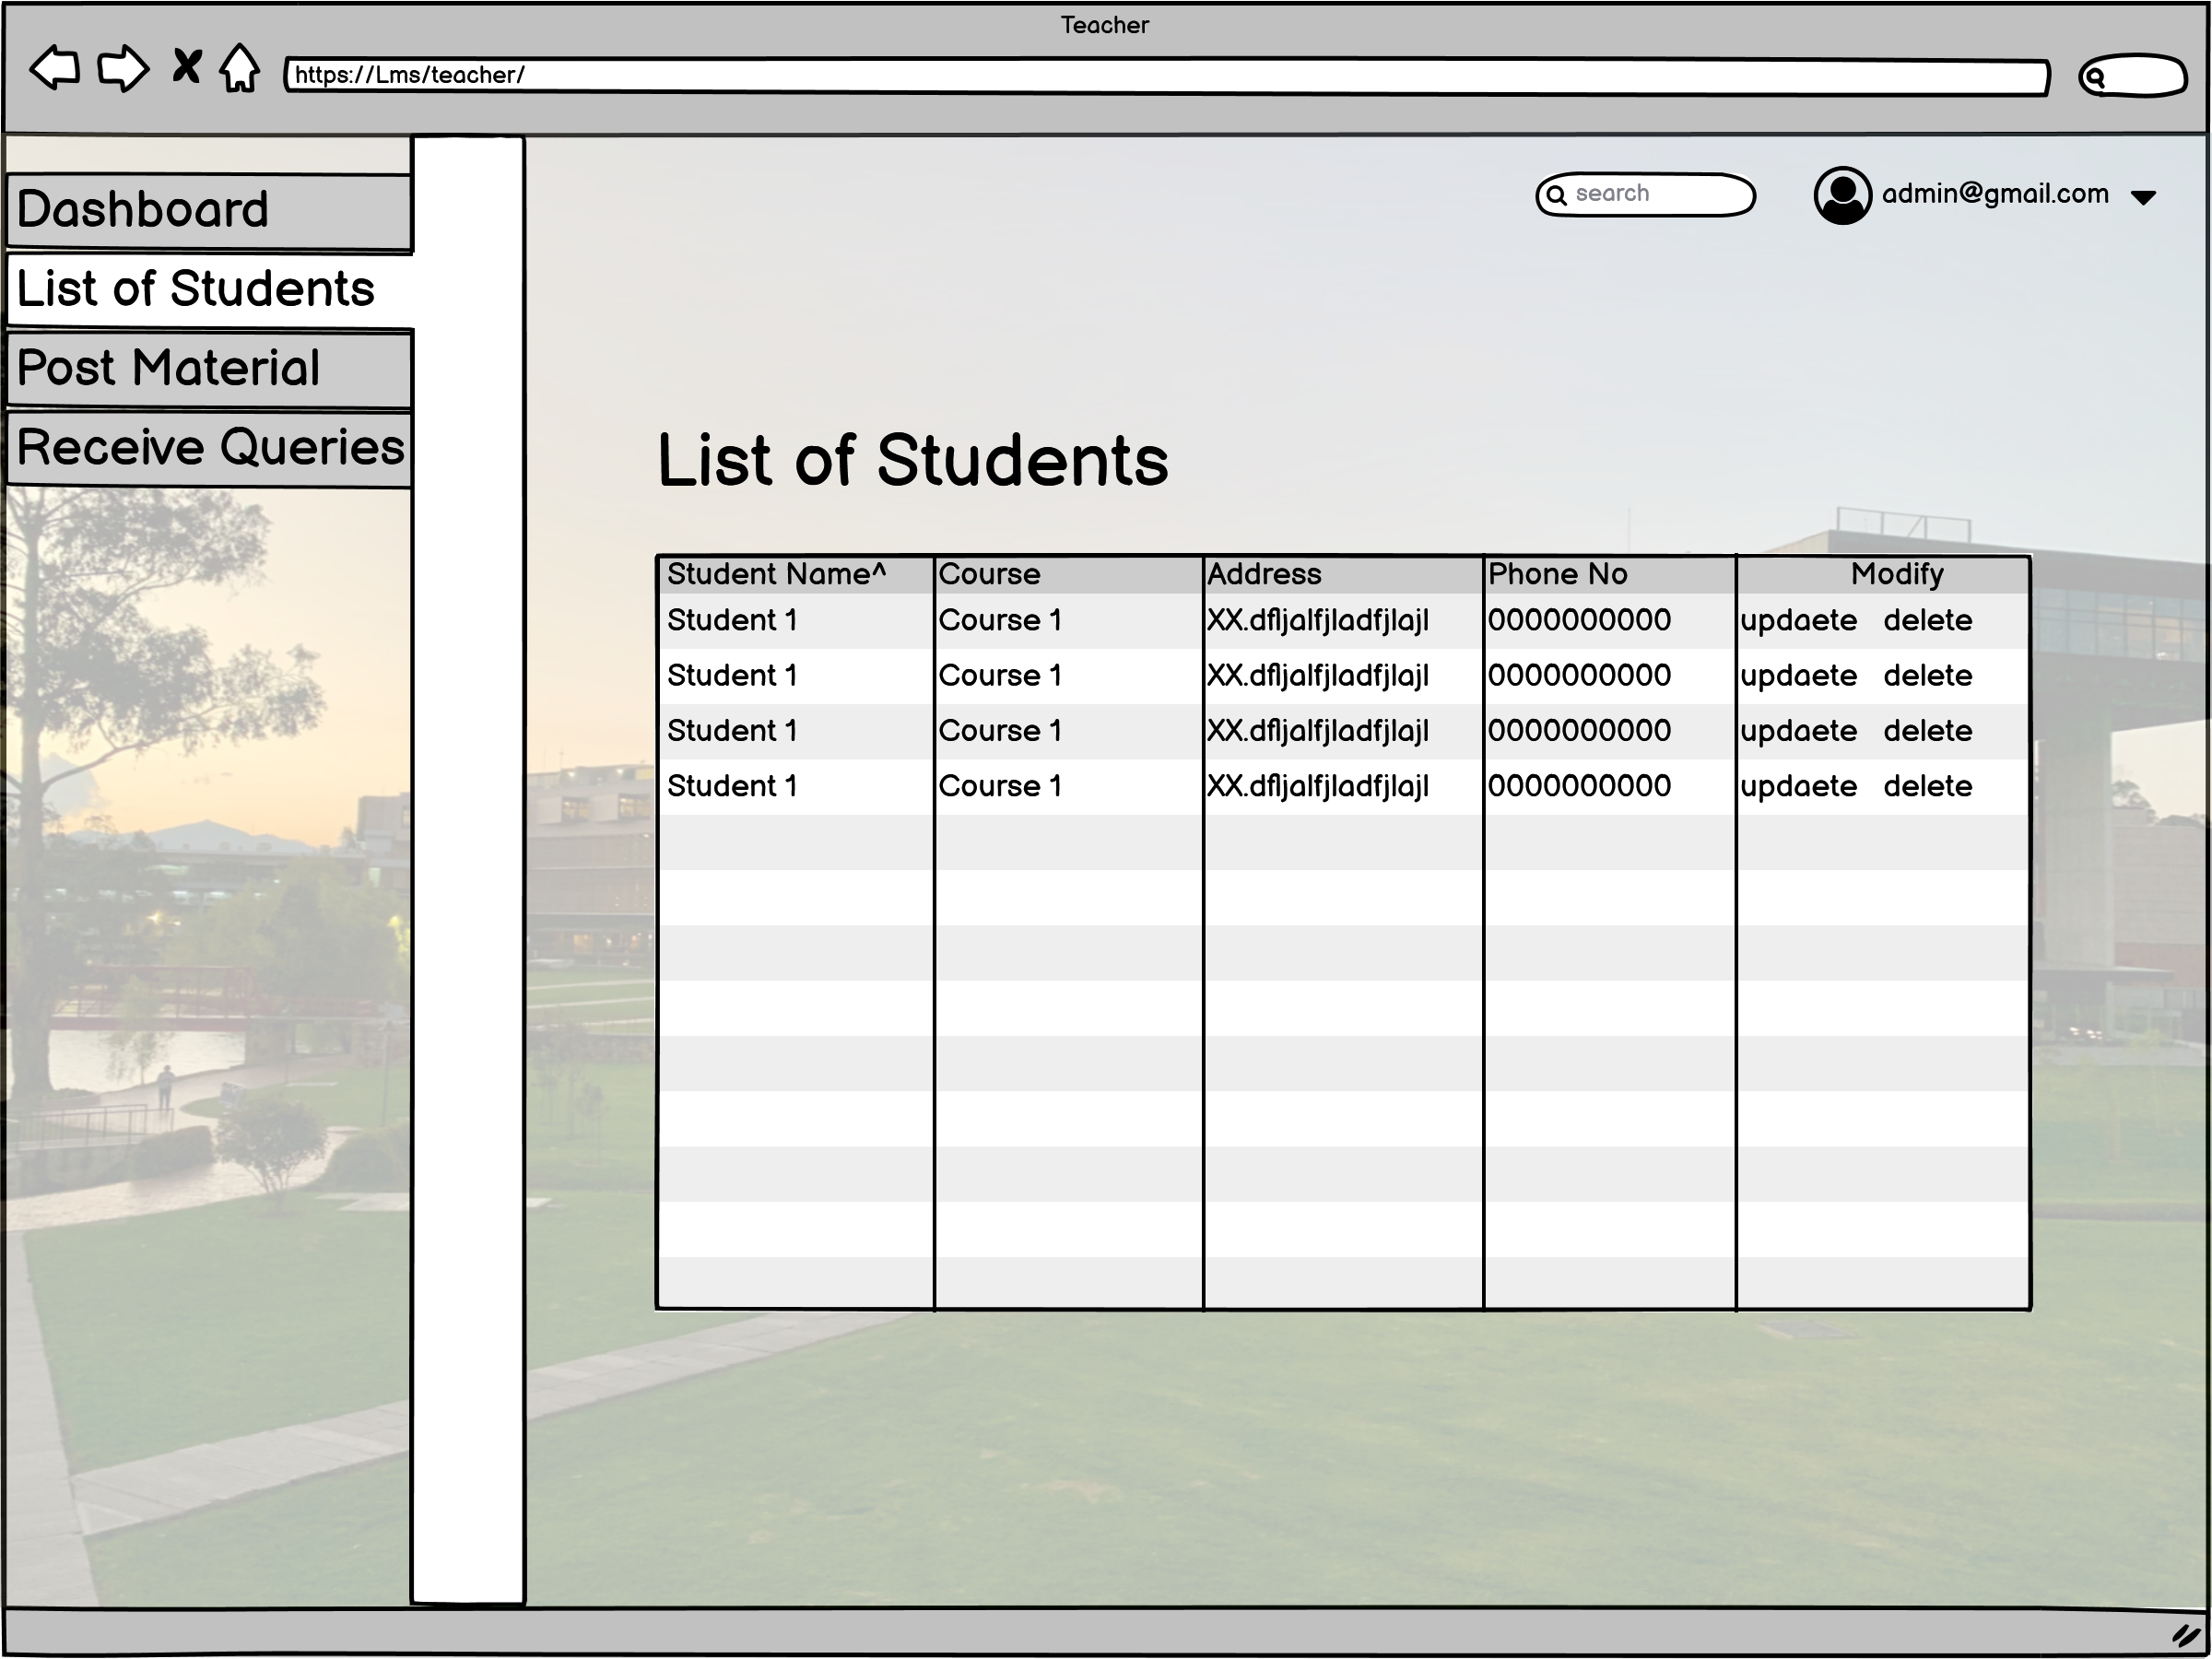
\includegraphics[width=\columnwidth]{images/List of Students teacher.png}
\newpage
The Post Material page contains a form for manual filling in the topic and description with uploading the necessary material. After the form is filled in the teacher posts it by clicking the “Send” button.\\

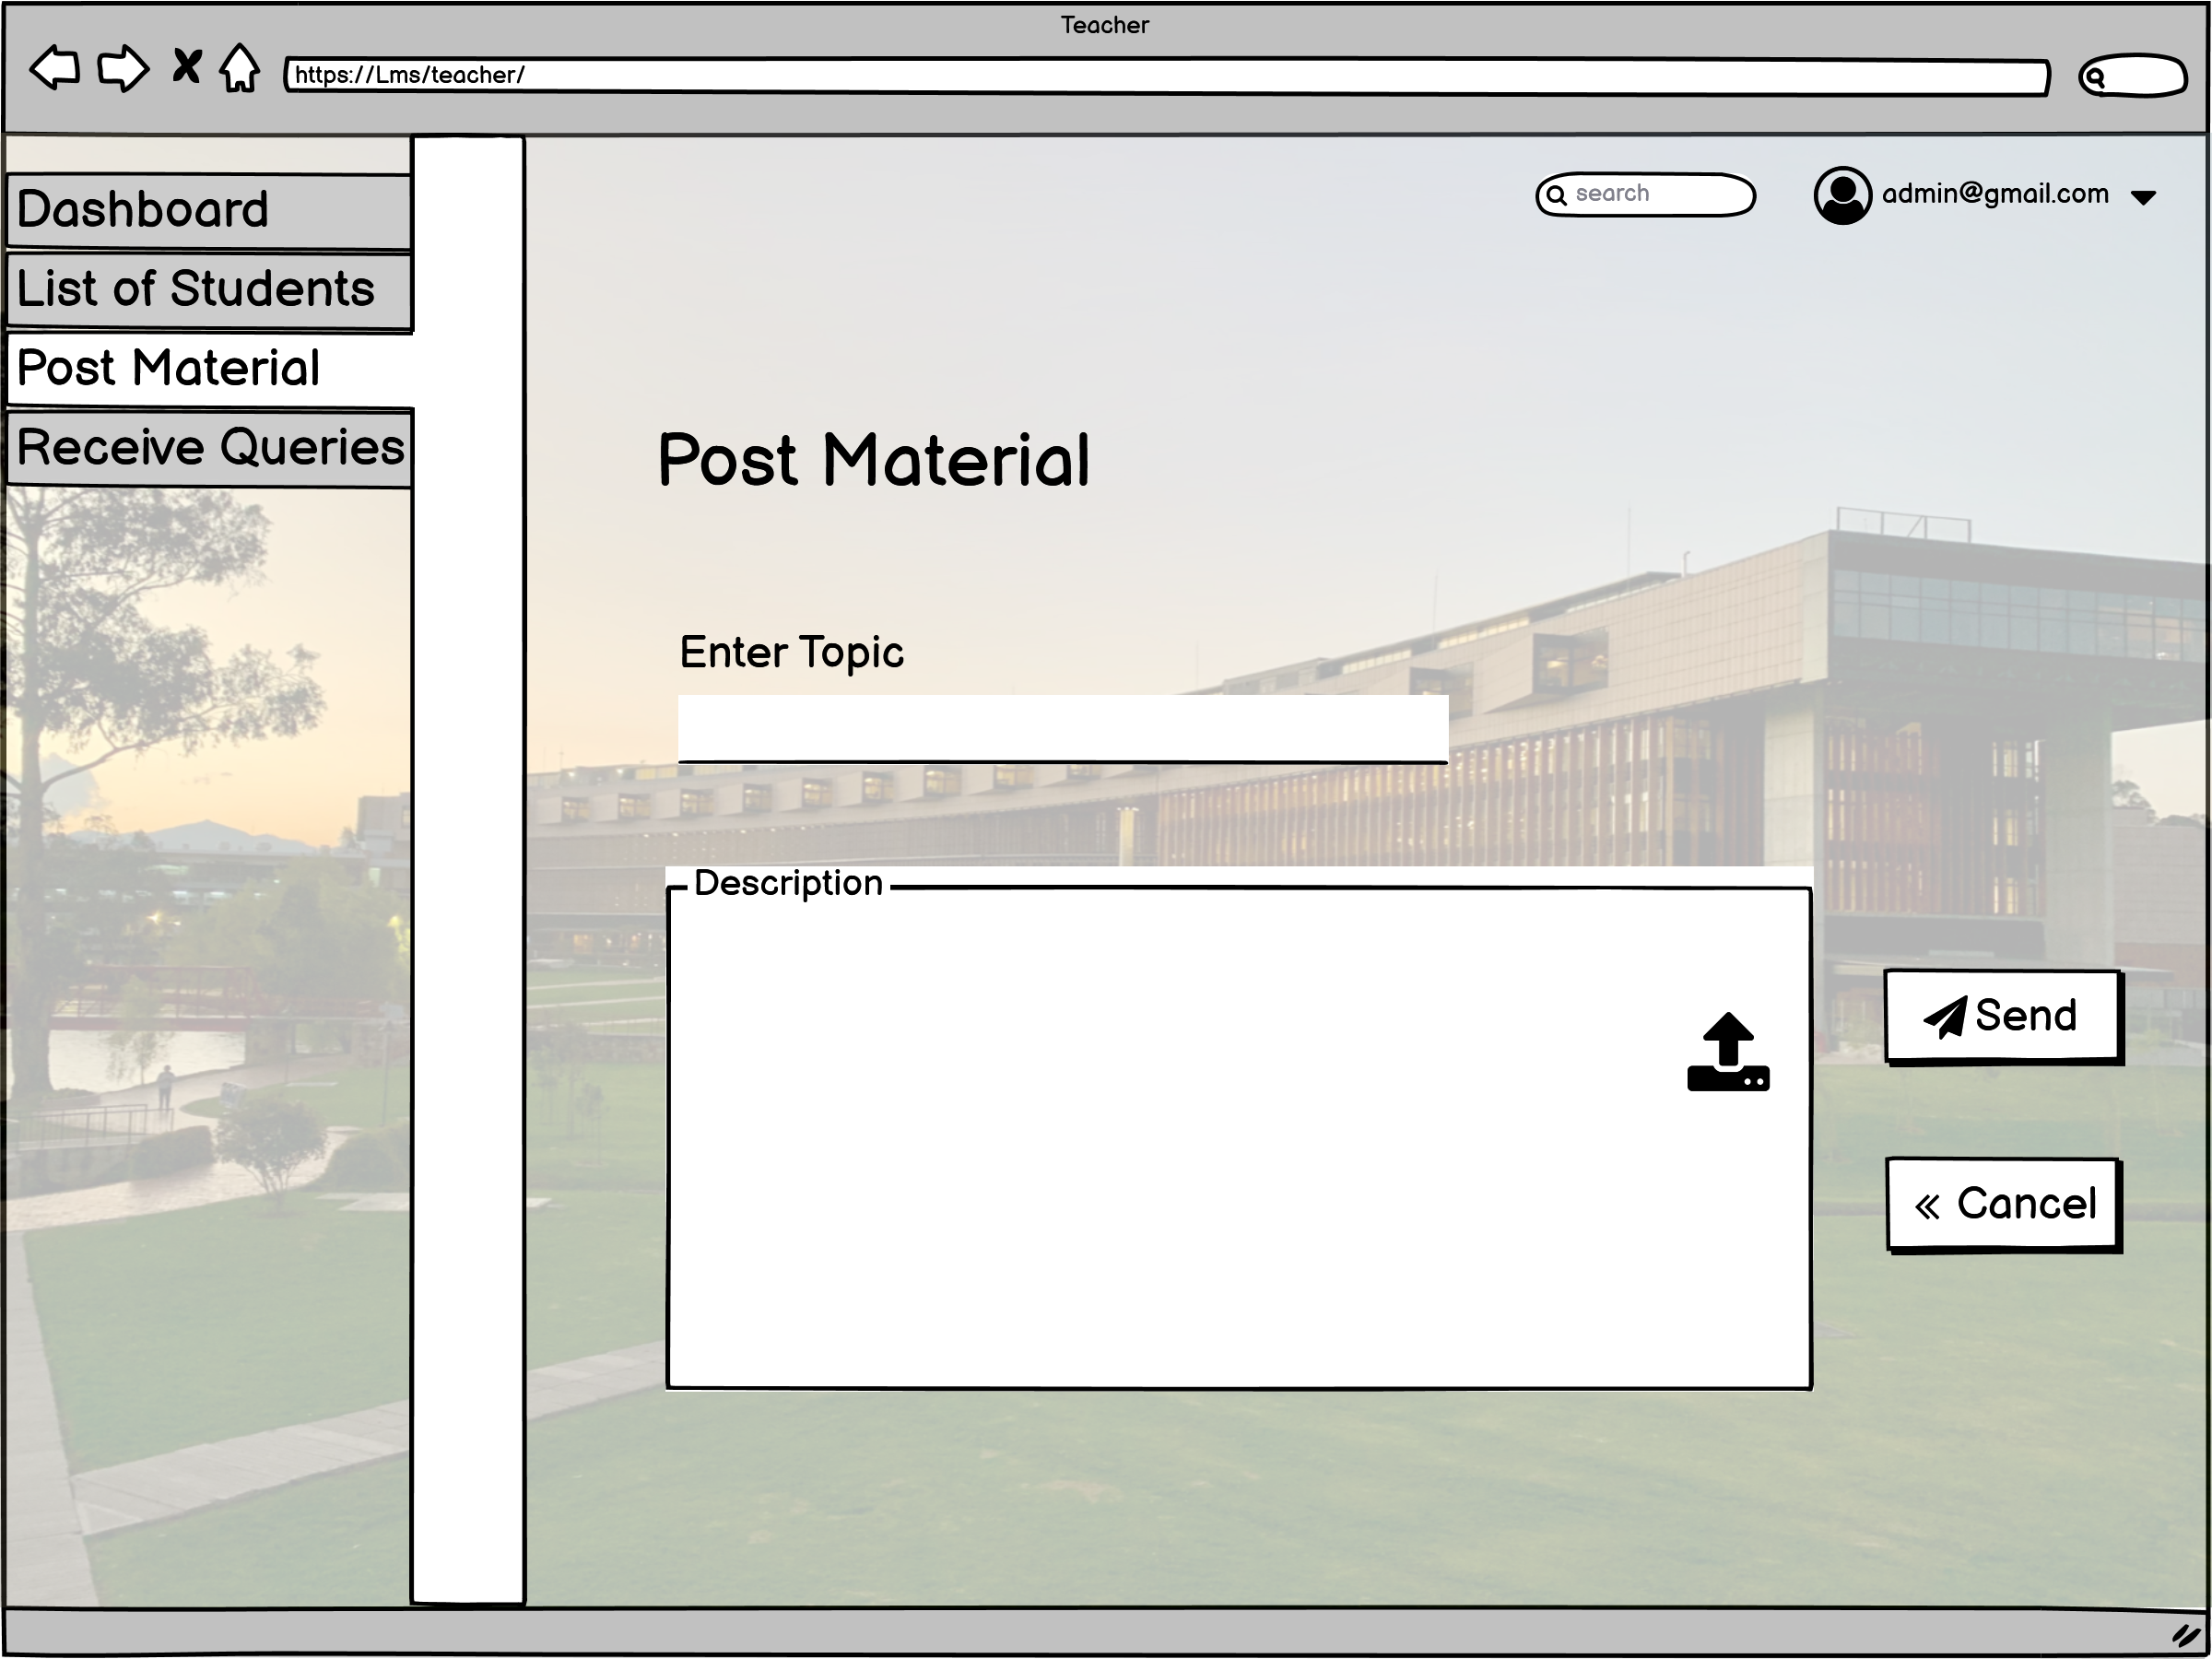
\includegraphics[width=\columnwidth]{images/Post Material.png}